\documentclass[bachelor]{cugthesis}

\usepackage{ttools}
\usepackage{tcode}

\cugthesistitle{中国地质大学研究生学位论文 \LaTeXe{} 模板}{\cugthesis\ \LaTeXe{} Template}
\studentid{1201711347}
\cugthesismajor{计算机科学与技术}{Earth Exploration and Information Technology}
\cugthesisteacher{蔡之华}{Zhihua Cai}
\cugthesisauthor{王震宇}{Zhenyu Wang}
\educatingunit{计算机学院}
\cugthesisdate{2018}{3}

\begin{document}

\cugabstract{
    本文是中国地质大学(武汉)研究生学位论文 \LaTeXe{} 模板的说明文档. 本文主要介绍了该模板的写作背景,
    写作目的, 使用方法, 以及稍微介绍一下此模板是如何写的, 当然也有鄙人写的一些小工具.
    本文也可以作为中国地质大学(武汉)
    研究生学位论文 \LaTeXe{} 模板的示例文件,
    因为本文内容基本上遵照了《中国地质大学(武汉)研究生学位论文写作规范》(2015年版).
}{This article is a description of the \LaTeXe{} template for a graduate dissertation of the 
                China University of Geosciences (Wuhan). This article mainly introduces
                The template's writing background, writing purpose, usages, and a little introduction about 
                how this template is written, of course there is also some useful utilities written by myself.
                This article can also be used as a \LaTeXe{} model for graduate students of the China University of Geosciences (Wuhan).
                the sample files for the board, because the content of this paper basically complies 
                with the ``Chinese University of Geosciences (Wuhan) Graduate Dissertation Writing Regulations
                Van ''(Version 2015).}

\cugkeywords{中国地质大学; 学位论文;  \LaTeX{} 模板; 研究生}{CUGThesis; \LaTeXe{} Template}

\makefrontpages 

\chapter{绪论}

\section{背景}
\label{sec:bei_jing_}
    请允许我先简单介绍一下 \TeX{}, \LaTeX{}, 
    因为可能很多人都没有听过这个软件, 自然就谈不上使用它了.
\subsection{什么是 \TeX{}?}
\label{sec:sub_what_is_tex_}
    \TeX{} 是由Donald Knuth 编写的一个基于低级编程语言的电子排版系统, 它能够对文章
    进行十分精美的排版.

    Donald Knuth 教授公开了他的全部源程序. \TeX{} 系统目前已经在数百种计算机系统上得到了
    实现, 也就是说不论你是使用 Windows 系统, Linux 系统, 还是 Mac OSX 系统, 你都可以使用
    \TeX{} 系统来对你写的文章进行排版. 

    \TeX{} 的强大之处在于其能够对文档的排版进行非常精细的控制, 这可以使你能够对你文章的每一处
    细节进行调整.

    \TeX{} 系统具有很好的稳定性, 目前可以说几乎没什么 BUG. 如果你在使用该系统的过程中真的发现了
    BUG, 你可以联系 Donald Knuth 教授提交反馈. 据说在报告 BUG 时你会获得一定的现金奖励.
\subsection{什么是 \LaTeX{}?}
\label{sec:sub_what_is_latex_}
    \LaTeX{} 是由 Leslie Lamport 开发的当今世界上最流行和使用最广泛的 \TeX{} 宏集. 它构筑在 PlainTeX
    的基础上, 并加进了很多的功能以使使用者可以更为方便的使用 \TeX{} 的功能. 因此, 即使使用者并不是
    很了解 \TeX{}, 也可以在短时间内生成高质量的文档. 对于复杂的数学公式, \LaTeX{} 的表现非常出色.

\subsection{\LaTeX{} 的优缺点}
\label{sec:sub_latex_advantages_disabvantages_}
缺点: 
\begin{itemize}
    \item 一般来说是不能在输入文章的同时看到最终的输出效果, 但是将文章用 \LaTeX{}编译之后, 可以在屏幕上预览最终的输出效果的; 
    \item 尽管在预先定义好的版面中可以调节一些参数, 设计全新的版面还是很困难的, 需要耗费大量的时间(这正是我要做的, 你不用担心); 
    \item 需要掌握一些\LaTeX{}的排版命令(很少一部分); 
    \item \LaTeX{}不适合于排版非结构化的、无序的文档; 
\end{itemize}

优点:
\begin{itemize}
    \item 提供专业级的排版设计, 使你的文档看起来如同印刷好的一样; 
    \item 可以更方便地排版数学公式; 
    \item 用户仅仅需要掌握少数容易理解的, 用来说明文档逻辑结构的命令, 而无需对实际的页面设计做胡乱的修补; 
    \item 可以很容易地生成脚注、索引、目录和参考文献等复杂的结构; 
    \item 有大量免费的可添加宏包, 协助你完成许多基本的LaTeX未直接支持的排版任务; 例如, 支持在文档中插入PostScript图形的宏包和排版符合各类标准的参考文献的宏包等; 
    \item \TeX{}作 \LaTeX{}的格式化引擎, 是免费软件并且具有极高的可移植性, 因此它几乎可以在任何硬件平台上运行; 
\end{itemize}
\subsection{我为什么开发这个模板?}
\subsubsection{原因一}
    在\ref{sec:sub_what_is_tex_}节中我们提到了 \TeX{} 可以对文档进行非常精细的控制, 但由此也造成了
    一个问题, 使用难度非常大, 导致了耗时耗力, 最后的效果还可能不是你想要的. 

    基于上面的问题, \LaTeX{} 对 \TeX{} 进行了一个封装, 使得其变得相对来说简单易用了一些. 但是对于
    从来没有使用过 \TeX{} 的人来说, 尤其是那些没有编程经验的人, 它还是非常的不友好. 

    因此, 我想在这里继续对其进行一个封装, 做成一个中国地质大学(武汉)研究生学位论文写作模板, 使得
    地大的研究生在写作过程中更容易一些, 把主要精力用在论文内容上, 而不是论文的排版格式. 

\subsubsection{原因二}
    目前网上是有一份中国地质大学(武汉)研究生学位论文 \LaTeX{} 模板\footnote{\url{https://github.com/xujinlai/CUGThesis}}的, 
    我看了一下, 作者是信息工程学院罗忠文教授的学生赵钱孙\footnote{我不知道这个是他的真名还是个
    文档内的示例名字, 如有所知者烦请告知, 我会更正本文档中的内容, 我的联系方式在表\ref{tab:contact}中可以查到. }
    于 2015 年 4 月份写的, 之后再没有再更新过. 可惜的是, 地大非常地不给面子, 于同年 12 月份修改了毕业论文的写作规范, 因此
    他的模板中的内容过时了, 不再适合使用了.
    
\subsubsection{原因三}
    在说原因三之前, 我首先要申明一下, 本文不是一个铁杆儿粉在专门提倡使用 \TeX{}, 也不是一个 Anti MSer 在
    大力宣传 Anti MS. 

    现在基本上每个人都在用 MS Word 做文字的排版, 尤其是高校学生, 经常要使用 MS Word 来写课程报告, 在毕业时候
    甚至还需要用它来做毕业设计论文的排版. 

    但是, 我想问一句, 你使用了这么多年 Word, 你真的会用吗? 你真的会用吗? 你真的会用吗? 

    仔细地思考一下我的问题. 我说的会用不包括 VisualBasicScript 编程, 这个毕竟是懂编程的人才会去研究的.

    返回头来看看你曾经写过的课程报告, 你觉得怎么样? 是版式排的非常漂亮, 还是烂的像一坨屎, 根本不能给人看?

    你自己满意吗?

    曾见过我的同学们是如何对课程报告进行排版的, 就是一个一个的字符调格式, 自动化工具不会用, 样式不会用,
    最后调了半天也没调出什么效果来, 仅仅是让人能区分出章节标题和正文了.

    我在这里说这个问题, 是想说, 我不是讨厌 Word, 而是讨厌从不知样式为何物"的 Word 用户, 这些人排版非常糟糕,
    ``不堪入目''.

    还有一个就是用 Word 排版非常低效, 即使你懂得如何使用 Word, 我是说懂得使用自动化工具和样式.

    总之一句话, 使用 \TeX{} 可以在极短的时间内做出最好的排版效果, 省时省力.

\section{目的}
\label{sec:mu_di_}
    在\ref{sec:sub_latex_advantages_disabvantages_}节中我们提到了 \LaTeX{} 设计全新的版面是困难的, 我想这点
    不用你操心, 我这不正是在给你做这个论文写作模板嘛, 不需要你自己设计.

    还有就是需要掌握一些 \LaTeX{} 排版命令, 关于这一点, 是系统本身带来的问题. 而我的目的呢, 就是尽量简化这些
    命令, 简化你的写作过程, 使你能够在使用相当少的命令的情况下得到相当漂亮的排版效果.

\section{问题反馈}
\label{sec:wen_ti_fan_kui_}
    本模板完全是由我一个人开发, 因此, 在写作过程中难免会出现各种错误, 或者是有些细节地方没有考虑到.

    因此, 如果你在使用模板的过程中如果有疑问, 遇到困难, 可以询问我, 我的联系方式可以在表\ref{tab:contact}中查到.
    
    如果你在使用过程中遇到了 BUG, 影响到了你的使用体验, 我在这里先向你说一句抱歉.
    然后诚恳地希望你可以给我一些反馈, 以便让该模板更好用. 当然, 如果您有一些建议, ideas 等, 也可以给我反馈. 
    请将反馈提交到
    \url{https://github.com/Timozer/CUGThesis/issues}中.


\chapter{使用方法}

\section{系统要求}
\label{sec:xi_tong_yao_qiu_}
本模板是基于 \CTeX{} 宏集中的 ctexbook 文档类进行定制的. 所以如果要使用该模板, 你必须
安装有 \CTeX{} 宏集. 我只知道 Texlive 完全安装包含了该宏集.

除了需要 ctexbook 文档类, 本模板还自动加载了一些必要和不必要的宏包, 如表\ref{tab:packagesautoload}
中所示. 因此你的电脑还必须安装有这些宏包, Texlive 完全安装会自动安装这些宏包.
\begin{ttab}{\cugthesis{} 自动加载的宏包}{tab:packagesautoload}
    \begin{tabular}{>{\bfseries}cl}
        \toprule 
        类别         & 宏包                                                         \\
        \midrule
        模板开发类   & xifthen, xparse, etoolbox                                    \\
        字体类       & xeCJK, fontsec                                               \\
        数学类       & amstext, amsmath, amssymb, amsfonts, mathrsfs, bm, mathtools \\
        插图类       & graphicx, subcaption                                         \\
        表格类       & array, longtable, makecell, tabu, booktabs                   \\
        列表类       & enumitem                                                     \\
        模板         & cugthesisfont                                                \\
        页面布局     & geometry                                                     \\
        目录样式     & tocloft                                                      \\
        超链接       & hyperref, url                                                \\
        浮动环境标题 & caption                                                      \\
        参考文献     & natbib                                                       \\
        \bottomrule
    \end{tabular}
\end{ttab}

本模板目前测试可以正常进行编译的系统环境如表\ref{tab:systems}所示.
\begin{ttab}{系统环境}{tab:systems}
    \begin{tabular}{cl}
        \toprule
        系统类别 & 编译环境            \\
        \midrule 
        Mac OSX  & Texlive2017:xelatex \\
        \bottomrule  
    \end{tabular}
\end{ttab}
\section{下载安装}
\label{sec:xia_zai_an_zhuang_}

\subsection{模板下载}
\label{sub:mo_ban_xia_zai_}
本模板是托管在 Github 上的一个项目, 项目地址: \url{https://github.com/Timozer/CUGThesis}. 你可以
在该网站上下载所有文件.

下载完整地址:

\url{https://github.com/Timozer/CUGThesis/archive/master.zip}

如果你使用 Linux 或者是 Mac OSX 系统, 你可以使用图形界面下载工具来下载, 也可以在终端中使用 wget 或者是 git 来
将它下载到本地. 如下:

\begin{minted}{sh}
wget https://github.com/Timozer/CUGThesis/archive/master.zip
# 或者是
git clone https://github.com/Timozer/CUGThesis.git 
\end{minted}

下载完成后请将压缩包解压, 然后清点一下文件, 看是否残缺, 本模板主要文件如表\ref{tab:templatefiles}所示.
\begin{ttab}{模板主要文件}{tab:templatefiles}
    \begin{tabular}{ll}
        \toprule
        文件名            & 说明                       \\
        \midrule
        cugthesis.cls     & 模板文档类主要文件         \\
        cugthesisfont.sty & 模板字体设置               \\
        authorcv.tex      & 作者简介                   \\
        gbt77140-2005.bst & 参考文献样式               \\
        demo.tex          & 本说明文档的 tex 源码文件  \\
        demo.pdf          & 本说明文档                 \\
        example.tex       & 示例源码文件               \\
        example.pdf       & 示例文档                   \\
        tex.bib           & 本文档引用的参考文献数据库 \\
        ttools.sty        & 小工具宏包                 \\
        tcode.sty         & 代码环境设置               \\
        LICENSE           & 协议文件                   \\
        README.md         & readme                     \\
        Makefile          & make 自动化工具所需文件    \\
        \bottomrule 
    \end{tabular}
\end{ttab}

\subsection{\LaTeX{}系统安装使用}
\label{sub:xi_tong_an_zhuang_shi_yong_}
\subsubsection{Windows \& Linux}
\label{ssub:Windows_Linux}
你可以在华科大开源镜像站获取到 texlive\footnote{\url{http://mirrors.ustc.edu.cn/CTAN/systems/texlive/Images/}}
的镜像文件.

\subsubsection{Mac OSX}
\label{ssub:Mac_OSX}
Mac 用户请使用 MacTex\footnote{\url{https://www.tug.org/mactex/}}.

%\begin{tfig}{MacTeX 下载首页}{fig:mactexdownload}
    %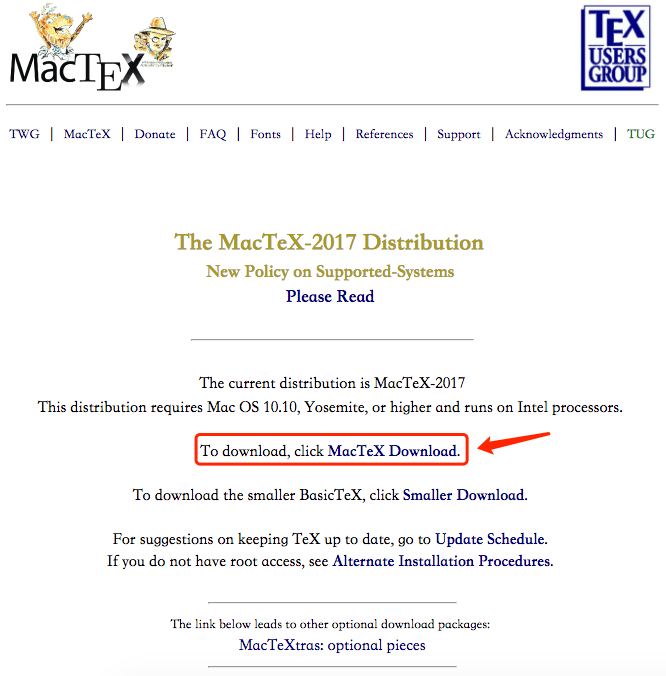
\includegraphics[width=\textwidth]{./imgs//mactexdownload.png}
%\end{tfig}

点击图中红色标出的链接, 进入下一页, 如图\ref{fig:mactexpkg}.

%\begin{tfig}{MacTeX pkg 下载}{fig:mactexpkg}
    %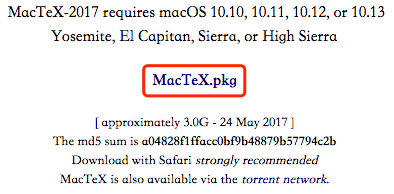
\includegraphics[width=.6\textwidth]{./imgs/mactexpkg.png}
%\end{tfig}

然后下载那个 pkg 安装包, 大约有 3.14 GB\@.
\section{模板基本使用}
\label{sec:mo_ban_ji_ben_shi_yong_}
要使用本模板, 您首先得具备基本的 \LaTeX{} 知识, 本模板的存在只是尽可能让你在
具备很少的知识的情况下做出精美的排版. 如果您刚刚接触 \LaTeX{}, 建议您先学习一下
相关的知识. 

什么? 您说啥? 没时间?

OK, 如果您没有很多时间来学习, 您可以先看看 The Not So Short Introduction to 
\LaTeXe{} \cite{oetiker_not_2018} 这篇文档, 大概占用您 139 分钟. 如果您觉得英文
读着费劲, 这里有一篇中文的《一份不太简短的 \LaTeXe{} 介绍》
\footnote{\url{http://ctan.math.illinois.edu/info/lshort/chinese/lshort-zh-cn.pdf}}.
读过这篇文档, 您基本已经会使用 \LaTeX{} 系统了. 接下来您就可以正常使用本模板了.
当然, 如果您在使用模板过程中对 \LaTeX{} 产生了兴趣, 想进一步了解, 您还可以读
《 \LaTeX{} 入门 》\cite{_latex_2013} 这本书.

下面步入正题.

本模板的文档类为 cugthesis, 为了方便使用, 您可以直接在该模板文件夹下创建自己的
文档.

你的文档一开始应该引入模板类, 就像下面这样:
\begin{minted}{tex}
    \documentclass[<option>]{cugthesis}
\end{minted}

本模板提供了一个选项, 意在表明你是什么学位, 博士还是硕士, 学硕还是专硕, 全日制还是
非全日制. 具体说明请查看表\ref{tab:classoptiondegree}.

\begin{ttab}{模板选项}{tab:classoptiondegree}
    \begin{tabular}{ll}
        \toprule
        文档选项            & 说明 \\
        \midrule
        doctor              & 博士 \\
        master              & 硕士 \\
        masterprofulltime   & 全日制专硕 \\
        masterpronofulltime & 非全日制专硕 \\
        \bottomrule
    \end{tabular}
\end{ttab}

比如说我是一个硕士, 我在使用的时候应该像下面这样:
\begin{minted}{tex}
    \documentclass[master]{cugthesis}
\end{minted}

在正确引入模板类后, 你就需要为你的论文添加一些相关信息了, 比如说论文题目, 论文作者, 
指导老师等.

模板为你提供了几个命令用来设置这些, 相关命令如表\ref{tab:cugthesisinfocmds}所示.
\begin{ttab}{论文相关信息命令}{tab:cugthesisinfocmds}
    \begin{tabular}{lll}
        \toprule
        命令 & 作用 & 用法 \\
        \midrule
        \tcodeinline{tex}{\cugthesistitle} & 论文标题 & \tcodeinline{tex}{\cugthesistitle{cntitle}{entitle}} \\
        \tcodeinline{tex}{\cugthesismajor} & 专业 & \tcodeinline{tex}{\cugthesismajor{cnmajor}{enmajor}} \\
        \tcodeinline{tex}{\cugthesisteacher} & 指导老师 & \tcodeinline{tex}{\cugthesisteacher{cnname}{enname}} \\
        \tcodeinline{tex}{\cugthesisauthor} &  作者姓名 & \tcodeinline{tex}{\cugthesisauthor{cnname}{enname}} \\
        \tcodeinline{tex}{\studentid} & 学号 & \tcodeinline{tex}{\studentid{1201711347}} \\
        \tcodeinline{tex}{\educatingunit} & 培养单位 & \tcodeinline{tex}{\educatingunit{计算机学院}} \\
        \tcodeinline{tex}{\cugthesisdate} & 时间 & \tcodeinline{tex}{\cugthesisdate{2018}{3}} \\
        \bottomrule
    \end{tabular}
\end{ttab}

然后你就应该像下面这样输入代码:
\begin{minted}{tex}
    \cugthesistitle{中国地质大学研究生学位论文 \LaTeXe{} 模板}{\cugthesis \LaTeXe{} 模板}
    \cugthesisauthor{王震宇}{Zhenyu Wang}
    \studentid{1201711347}
    \cugthesismajor{计算机科学与技术}{Computer Science}
    \cugthesisteacher{蔡之华}{Zhihua Cai}
    \educatingunit{计算机学院}
    \cugthesisdate{2018}{3}
\end{minted}

顺序无关紧要, 你可以根据你的喜好随意安排.

然后就是开始你的正文了. 请将你的正文放入 document 环境中, 如下:
\begin{minted}{tex}
    \begin{document}
        % 你的正文
    \end{document}
\end{minted}

你的论文的摘要, 关键字等可以通过模板提供的相关命令来写, 具体命令如表\ref{tab:abstractcmds}所示.
\begin{ttab}{摘要相关命令}{tab:abstractcmds}
    \begin{tabular}{ll}
        \toprule
        命令 & 用法 \\
        \midrule
        \tcodeinline{tex}{\cugabstract} & \tcodeinline{tex}{\cugabstract{这里是中文摘要}{Here is english abstract}} \\
        \tcodeinline{tex}{\cugkeywords} & \tcodeinline{tex}{\cugkeywords{关键字}{Keywords}} \\
        \bottomrule
    \end{tabular}
\end{ttab}

你的摘要应该像下面这样:
\begin{minted}{tex}
    \cugabstract{中文摘要}{English Abstract}
    \cugkeywords{关键字}{Keywords} 
\end{minted}

接下来就是让 \LaTeX{} 生成论文正文前面的这些页面了, 比如说题名页, 原创性声明, 导师承诺书, 授权书, 摘要,
目录, 插图清单, 表格清单等.
你可以使用\tcodeinline{tex}{\makefrontpages}来生成. 这个是模板提供的命令.

然后你就开始写你的正文. 当你的正文写完后, 需要些致谢, 参考文献这些的时候, 需要用\tcodeinline{tex}{\backmatter}
命令来开启章节不编号功能. 当你需要为你的论文添加附录的时候, 你需要使用\tcodeinline{tex}{\appendix}命令来开启
章节字母编号功能.

最后, 你的整个论文源码应该类似下面这样:
\begin{minted}{tex}
    \documentclass[master]{cugthesis}

    \cugthesistitle{中国地质大学研究生学位论文 \LaTeXe{} 模板}{\cugthesis \LaTeXe{} 模板}
    \cugthesisauthor{王震宇}{Zhenyu Wang}
    \studentid{1201711347}
    \cugthesismajor{计算机科学与技术}{Computer Science}
    \cugthesisteacher{蔡之华}{Zhihua Cai}
    \educatingunit{计算机学院}
    \cugthesisdate{2018}{3}

    \begin{document}
        \cugabstract{中文摘要}{English Abstract}
        \cugkeywords{关键字}{Keywords} 
        \makefrontpages 
        % 你的正文
        \chapter{这是第一章}
            % 更多内容
        \section{这是一级标题}
            % 更多内容
        \subsection{这是二级标题}
            % 更多内容

        \backmatter
        \chapter{致谢}
            % 致谢内容
        \cugthesisbib{参考文献数据库文件名}

        \appendix
        \chapter{这是附录A}
            % 这里是附录内容
    \end{document}
\end{minted}

基本使用说明到此为止, 祝您好运!

\chapter{正文排版建议以及一些示例}

\section{字体}
\label{sec:zi_ti_}


\section{标点符号}
\label{sec:biao_dian_fu_hao_}


\section{数学公式}
\label{sec:shu_xue_gong_shi_}

\subsection{公式环境建议}
\label{sub:gong_shi_huan_jing_jian_yi_}

在 \LaTeX{} 中插入数学公式有很多种方法, 包括行内公式和行间公式. 在这里根据我的使用经验, 给你提供一些建议.

%如果你想插入行内公式, 请使用\$公式\$, 虽然$\backslash($和$\backslash)$也能实现插入行内公式, 
如果你想插入行内公式, 请使用 \tilcode{\textbackslash(~\ldots~\textbackslash)}, 尽量不要使用 \tilcode{\$~\ldots~\$}.
前者是 \LaTeX{} 中的符号, 后者是 \TeX{} 中的符号. 尽管你可以在 \LaTeX{} 中两者都使用, 但是当你在公式里面
出现错误的时候, 前者不会给你太多费解的错误提示信息.

但是你也要注意, \tilcode{\textbackslash(~\ldots~\textbackslash)} 是个 \emph{fragile} 命令, 不能用在章节标题中.
当然如果你觉得你的公式不会出现错误, 你可以使用 \tilcode{\$~\ldots~\$}, 毕竟简洁清晰.

下面给出 \tilcode{\textbackslash(} 和 \tilcode{\textbackslash)} 在 \LaTeX{} 中的定义, 体会一下不同.
\begin{minted}{tex}
    \DeclareRobustCommand\({%
      \relax\ifmmode\@badmath\else$\fi}%
    \DeclareRobustCommand\){%
      \relax\ifmmode\ifinner$\else\@badmath\fi\else\@badmath\fi}%
\end{minted}

更多关于他们之间的讨论请参考脚注中提到的链接\footnote{\url{https://tex.stackexchange.com/questions/510/are-and-preferable-to-dollar-signs-for-math-mode}}.

如果你想插入行间公式, 请使用 \tilcode{\textbackslash begin\{equation\}~\dots~\textbackslash end\{equation\}}. 
尽管你可以使用 \tilcode{\$\$~\dots~\$\$} 或者是 \tilcode{\textbackslash[~\dots~\textbackslash]}, 但是
在你的论文中肯定是需要给公式编号的, 用 \tilcode{equation} 公式环境容易实现公式编号, 其他两个能不能
实现编号, 如何实现编号, 我不知道, 我也懒得去研究.

{\noindent
\begin{minipage}{.6\textwidth}
    \begin{minted}{tex}
        $$
            E = mc^{2}
        $$
    \end{minted}
\end{minipage}%
\begin{minipage}{.4\textwidth}
    $$
        E = mc^{2}
    $$
\end{minipage}
}

{\noindent
\begin{minipage}{.6\textwidth}
    \begin{minted}{tex}
        \[
            E = mc^{2}
        \]
    \end{minted}
\end{minipage}%
\begin{minipage}{.4\textwidth}
    \[
        E = mc^{2}
    \]
\end{minipage}
}

{\noindent
\begin{minipage}{.6\textwidth}
    \begin{minted}{tex}
        \begin{equation}
            E = mc^{2}
        \end{equation}
    \end{minted}
\end{minipage}%
\begin{minipage}{.4\textwidth}
        \begin{equation}
            E = mc^{2}
        \end{equation}
\end{minipage}
}

更多关于这方面的讨论请参考脚注中的链接\footnote{\url{https://tex.stackexchange.com/questions/503/why-is-preferable-to}}.

\subsection{公式排版建议}
\label{sub:gong_shi_pai_ban_jian_yi_}


\section{插图}
\label{sec:cha_tu_}

\section{表格}
\label{sec:biao_ge_}


\section{参考文献}
\label{sec:can_kao_wen_xian_}

本模板引入参考文献的命令是\tcodeinline{tex}{\cugthesisbib{bib_file_name}}.
会自动添加 ``参考文献'' 章节标题以及目录项, 所以不用你额外再写诸如\tcodeinline{tex}{\chapter{参考文献}}之类的代码.

\emph{bib\_file\_name} 是指你的参考文献数据库. 

关于参考文献数据库你可以自己手动录入, 也可以使用工具自动生成. 比如说 Zotero, JabRef, Mendeley 这些参考文献
管理工具. 如图\ref{fig:bibtoolexport}所示是我用 Zotero 导出文献引用数据.
%\begin{tfig}{Zotero导出参考文献引用数据}{fig:bibtoolexport}
    %\begin{minipage}{.66\textwidth}
        %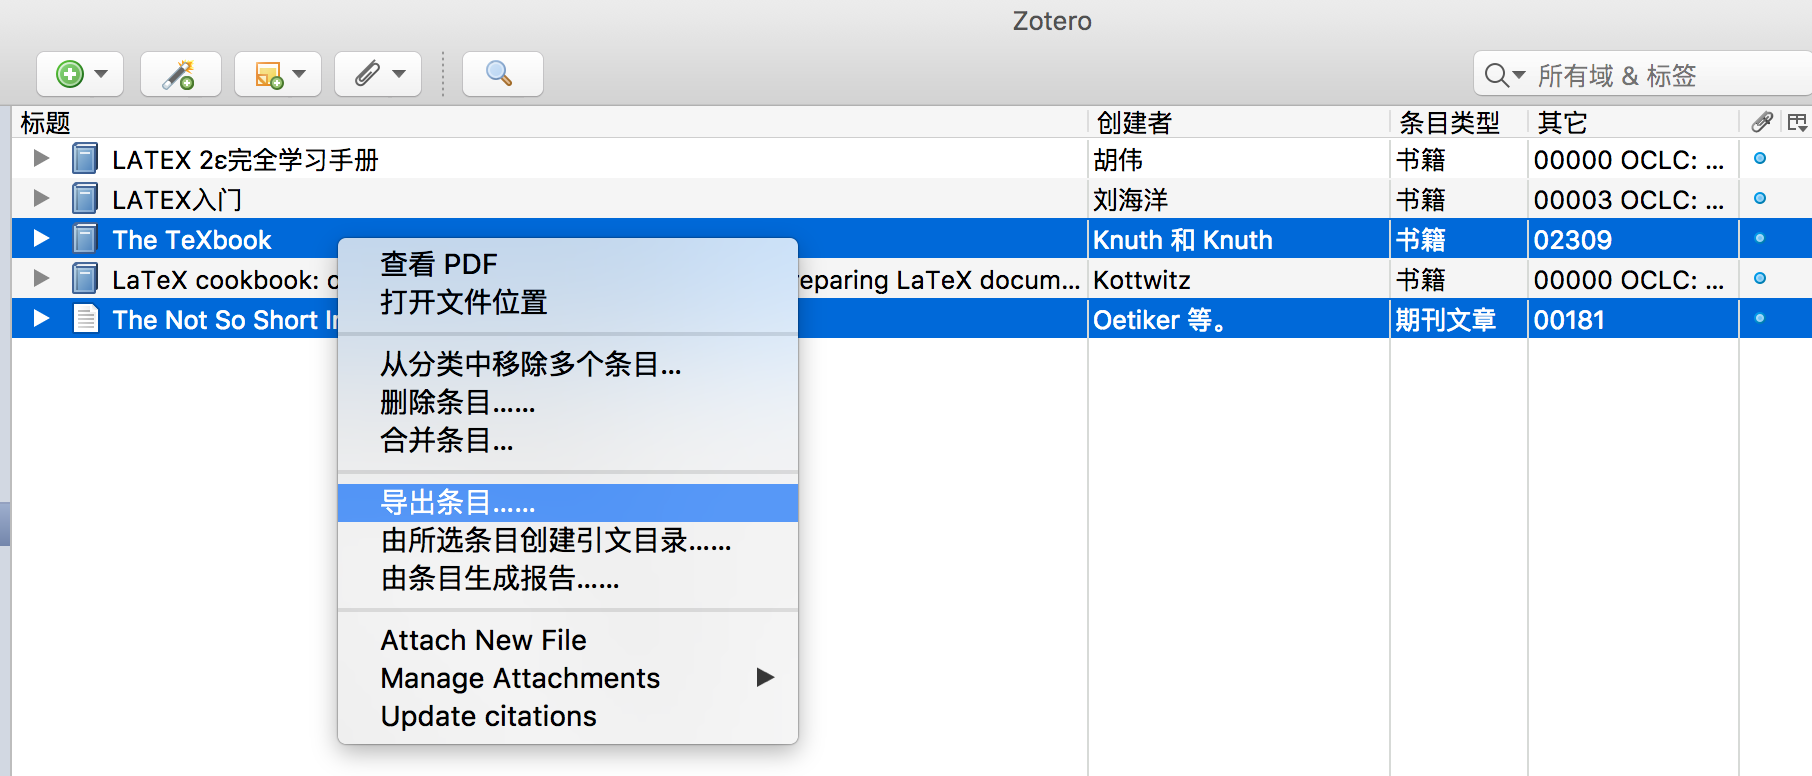
\includegraphics[width=\textwidth]{./imgs/zoteroexport1.png}
    %\end{minipage}%
    %\begin{minipage}{.33\textwidth}
        %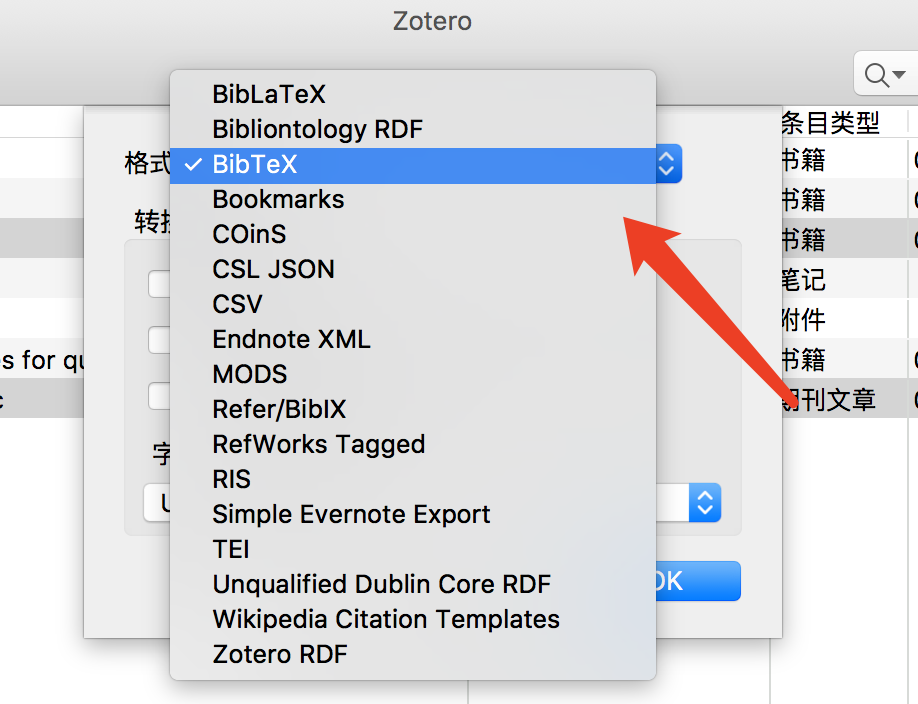
\includegraphics[width=\textwidth]{./imgs/zoteroexportbibtex.png}
    %\end{minipage}
%\end{tfig}

你也可以在下载参考文献的时候下载其对应的 cite key, 如图\ref{fig:bibcitekey}. 
%\begin{tfig}{文献 bibtex}{fig:bibcitekey}
    %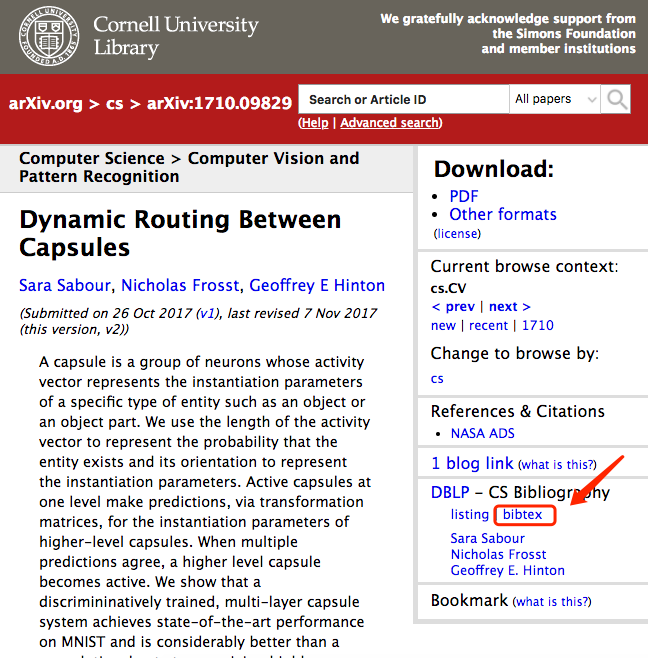
\includegraphics[width=.7\textwidth]{./imgs/papercitekey.png}
%\end{tfig}
\chapter{Utilities}

\chapter{实现}

\chapter{更新日志}

\section{Version 0.1}
\label{sec:version_0_1}

2018年 3月14日 星期三 14时05分07秒 CST

本模板从12日着手准备开发, 到现在已经将论文所要求的页面已经基本实现了, 除了作者简介页面和参考文献.
虽然页面基本实现了, 而且一些格式也设置了, 但仍然没有达到论文规范的要求, 因此在接下来的版本中我
会逐渐将没有实现的实现了, 把格式都调好了.

TODO list:
\begin{itemize}
    \item 题名页, 原创声明, 导师承诺书, 授权书, 摘要这些页面继续调整一下, 让人看起来更舒服一些;
    \item 目录格式;
    \item 关于论文中字体格式的调整;
    \item 模板使用字体的选择;
    \item 小工具的编写;
    \item 还没想好\dots
\end{itemize}

2018年 3月15日 星期四 11时18分01秒 CST

修正字号, 因为正文默认使用小四字体, 即在 \CTeX{} 中设置为 12pt, 所以关于 Huge, huge, LARGE 等这些命令
所对应的字体变大了. 而之前使用的定义有误, 所以重新定义字号大小.

设置目录的格式完成. 关于目录的格式问题: 规范里要求一级节标题和二级节标题左缩进一个汉字和两个汉字的距离,
但是章标题和节标题的字号大小却不一样, 所以排版出的效果不是很好. 因此, 我擅自将一级节标题的缩进改为 1.2
个汉字, 二级节标题改为 2.5 个汉字. 

TODO list:
\begin{itemize}
    \item 模板使用字体的选择;
    \item 小工具的编写;
    \item 说明文档的完善;
    \item 简介页面的制作;
    \item 参考文献页面的制作;
    \item 还没想好\dots
\end{itemize}

OK, 目前这个版本实现的功能就是这么多, 其他功能下个版本再添加. 

\section{Version 0.2}
\label{sec:version_0_2}
初步完成了简历页面的制作, 模板使用字体暂时就这些吧.

该版本已经基本完成, 目前已经是一个可以使用的模板了, 不过说明文档的欠缺, 使得
在使用时有一定的难度. 之后我会慢慢的补充文档, 编程好的同学可以自己查看我的
类文档, 来获得使用方法.

Developed!

\section{Versino 0.3}
\label{sec:versino_0_3}

2018年 3月16日 星期五 18时44分24秒 CST

这一版本中主要是完善说明文档, 基本将第二章写完了.

在更新说明文档的过程中, 又对模板类进行了一次结构优化, 使用在使用的过程中需要输入
的代码量更少, 这样大大简化了论文写作过程, 是作者专注于论文的内容, 而不是各种各样
内容标记代码.

此外, 这一版在写说明文档的时候还附带了写了一个简化代码的小工具. 比如说插图和表格,
在论文写作规范中要求标题的位置不同, 你自己使用浮动体环境的时候需要自己有意设置标题位置,
对此我做了一个封装, 使得你不用关心他们的标题到底应该放在哪儿.

还在交叉引用的标号左右增加了一点距离, 使得看起来更美观.

2018年 3月17日 星期六 14时36分07秒 CST

修正一个页眉的错误, 奇数页页眉要求是要显示博士学位论文, 硕士学位论文这几个字的. 我
之前看的是附件, 没有主要到这一要求.

修正一个BUG\@. 博士选项开启时候会出现一个问题, 已经解决了.

2018年 3月17日 星期六 22时53分42秒 CST

痛定思痛后终于下定决心换字体了, \CTeX{} 默认设置的字体也太难看了. 我将宋体和黑体换成了
思源宋体和思源黑体.

这两款字体免费的, 在使用的时候不需要考虑版权的问题. 下载地址见脚注\footnote{\url{https://github.com/adobe-fonts}}.

2018年 3月19日 星期一 09时13分52秒 CST

代码测试: \tilcode{\$~\dots~\$}
\backmatter{}
\cugthesisacknowledgements

%\chapter{致谢}

% 这里是参考文献
\cugthesisbib{tex}

\appendix
\chapter{文档示例}
\label{chapter:egdoc}

这里我将示例文档的内容插入进来, 以供大家查看.

\begin{table}[htpb]
    \centering
    \caption{联系方式}
    \label{tab:contact}
    \begin{tabular}{>{\sffamily}l>{\ttfamily\small}l}
        \toprule
        E-mail & zhenyuwang94@gmail.com \\
        QQ & 878592748 \\
        Github & \url{https://github.com/Timozer} \\
        \bottomrule 
    \end{tabular}
\end{table}

不管用何种方式联系我, 请注明 ``CUGThesis 模板问题''.

\chapter{LICENSE}
\cugthesis 模板采用的是 GPLv3 协议, 下面给出简短说明, 详情请参看目录下的 LICENSE 文件.

Copyright © 2018 Timozer <zhenyuwang94@gmail.com>

This program is free software: you can redistribute it and/or modify
it under the terms of the GNU General Public License as published by
the Free Software Foundation, either version 3 of the License, or
(at your option) any later version.

This program is distributed in the hope that it will be useful,
but WITHOUT ANY WARRANTY; without even the implied warranty of
MERCHANTABILITY or FITNESS FOR A PARTICULAR PURPOSE.  See the
GNU General Public License for more details.

You should have received a copy of the GNU General Public License
along with this program.  If not, see <\url{http://www.gnu.org/licenses}/>.

\end{document}
